\documentclass[11pt,letterpaper]{article}

% =============================================================================
% PACKAGES
% =============================================================================
\usepackage[margin=1in]{geometry}
\usepackage{enumitem}
\usepackage{setspace}
\usepackage{graphicx}
\usepackage{xcolor}
\usepackage{tikz}
\usetikzlibrary{shapes.geometric, arrows.meta, positioning, fit, backgrounds, calc, decorations.pathreplacing, trees, matrix, shapes.multipart, shapes.symbols, shadows, chains}
\usepackage{tcolorbox}
\usepackage{booktabs}
\usepackage{longtable}
\usepackage{array}
\usepackage{tabularx}
\usepackage{multirow}
\usepackage{colortbl}
\usepackage{fancyhdr}
\usepackage{titlesec}
\usepackage[colorlinks=true,linkcolor=blue!60!black,urlcolor=blue!60!black,citecolor=blue!60!black]{hyperref}
\usepackage{bookmark}
\usepackage{parskip}
\usepackage{float}
\usepackage{caption}
\usepackage{subcaption}
\usepackage{listings}
\usepackage{textcomp}
\usepackage{amssymb}
\usepackage{amsmath}
\usepackage{pifont}

% =============================================================================
% CONFIGURATION
% =============================================================================
\setstretch{1.15}

% Define colors
\definecolor{primary}{RGB}{60, 110, 60}
\definecolor{secondary}{RGB}{90, 140, 90}
\definecolor{accent}{RGB}{200, 120, 50}
\definecolor{success}{RGB}{50, 150, 80}
\definecolor{warning}{RGB}{220, 170, 50}
\definecolor{critical}{RGB}{190, 60, 60}
\definecolor{lightgray}{RGB}{245, 245, 245}
\definecolor{darkgray}{RGB}{80, 80, 80}
\definecolor{pipelinecolor}{RGB}{230, 245, 235}
\definecolor{artifactcolor}{RGB}{255, 245, 230}
\definecolor{testcolor}{RGB}{235, 240, 255}
\definecolor{deploycolor}{RGB}{255, 235, 235}
\definecolor{sourcecolor}{RGB}{245, 240, 255}
\definecolor{qualitycolor}{RGB}{240, 255, 245}
\definecolor{stagecolor}{RGB}{220, 235, 250}

% Section formatting
\titleformat{\section}{\Large\bfseries\color{primary}}{\thesection}{1em}{}[\titlerule]
\titleformat{\subsection}{\large\bfseries\color{secondary}}{\thesubsection}{1em}{}
\titleformat{\subsubsection}{\normalsize\bfseries\color{darkgray}}{\thesubsubsection}{1em}{}

% Header/Footer
\pagestyle{fancy}
\fancyhf{}
\fancyhead[L]{\small\textcolor{darkgray}{Builder's View Specification}}
\fancyhead[R]{\small\textcolor{darkgray}{Architecture Documentation}}
\fancyfoot[C]{\thepage}
\renewcommand{\headrulewidth}{0.4pt}

% Custom environments
\newtcolorbox{definitionbox}[1][]{
    colback=lightgray,
    colframe=primary,
    fonttitle=\bfseries,
    title=#1,
    boxrule=0.5pt,
    arc=2pt,
    left=8pt,
    right=8pt,
    top=6pt,
    bottom=6pt
}

\newtcolorbox{examplebox}[1][]{
    colback=white,
    colframe=secondary,
    fonttitle=\bfseries,
    title=#1,
    boxrule=0.5pt,
    arc=2pt,
    left=8pt,
    right=8pt,
    top=6pt,
    bottom=6pt
}

\newtcolorbox{warningbox}[1][]{
    colback=orange!5,
    colframe=accent,
    fonttitle=\bfseries,
    title=#1,
    boxrule=0.5pt,
    arc=2pt,
    left=8pt,
    right=8pt,
    top=6pt,
    bottom=6pt
}

\newtcolorbox{guidancebox}[1][]{
    colback=green!5,
    colframe=success,
    fonttitle=\bfseries,
    title=#1,
    boxrule=0.5pt,
    arc=2pt,
    left=8pt,
    right=8pt,
    top=6pt,
    bottom=6pt
}

\newtcolorbox{patternbox}[1][]{
    colback=blue!3,
    colframe=primary!70,
    fonttitle=\bfseries,
    title=#1,
    boxrule=0.5pt,
    arc=2pt,
    left=8pt,
    right=8pt,
    top=6pt,
    bottom=6pt
}

\newtcolorbox{pipelinebox}[1][]{
    colback=green!5,
    colframe=primary,
    fonttitle=\bfseries,
    title=#1,
    boxrule=0.5pt,
    arc=2pt,
    left=8pt,
    right=8pt,
    top=6pt,
    bottom=6pt
}

\newtcolorbox{artifactbox}[1][]{
    colback=orange!5,
    colframe=accent!80,
    fonttitle=\bfseries,
    title=#1,
    boxrule=0.5pt,
    arc=2pt,
    left=8pt,
    right=8pt,
    top=6pt,
    bottom=6pt
}

\newtcolorbox{qualitybox}[1][]{
    colback=blue!5,
    colframe=secondary!80,
    fonttitle=\bfseries,
    title=#1,
    boxrule=0.5pt,
    arc=2pt,
    left=8pt,
    right=8pt,
    top=6pt,
    bottom=6pt
}

% Listings configuration
% NOTE: The `listings` package does not ship with a built-in YAML language.
% Define a lightweight YAML lexer so `language=yaml` blocks compile cleanly.
\lstdefinelanguage{yaml}{
    sensitive=false,
    comment=[l]{\#},
    morestring=[b]',
    morestring=[b]",
    alsoletter={-},
    keywords={true,false,null,yes,no,on,off},
}

\lstset{
    basicstyle=\ttfamily\small,
    backgroundcolor=\color{lightgray},
    frame=single,
    framerule=0.5pt,
    rulecolor=\color{darkgray},
    breaklines=true,
    captionpos=b,
    tabsize=2,
    showstringspaces=false,
    numbers=left,
    numberstyle=\tiny\color{darkgray},
    numbersep=5pt,
    xleftmargin=15pt,
    keywordstyle=\color{primary}\bfseries,
    commentstyle=\color{darkgray}\itshape,
    stringstyle=\color{success},
    morekeywords={stage, steps, script, when, environment, agent, pipeline, job, runs-on, uses, with, needs, if, name, on, push, pull_request}
}

% Table column types
\newcolumntype{L}[1]{>{\raggedright\arraybackslash}p{#1}}
\newcolumntype{C}[1]{>{\centering\arraybackslash}p{#1}}
\newcolumntype{R}[1]{>{\raggedleft\arraybackslash}p{#1}}

% Custom commands
\newcommand{\cmark}{\ding{51}}
\newcommand{\xmark}{\ding{55}}

% =============================================================================
% DOCUMENT BEGIN
% =============================================================================
\begin{document}

% -----------------------------------------------------------------------------
% TITLE PAGE
% -----------------------------------------------------------------------------
% Avoid duplicate PDF destinations when the titlepage environment resets the page
% counter (hyperref anchors page.1 twice otherwise).
\hypersetup{pageanchor=false}
\begin{titlepage}
    \centering
    \vspace*{1.5cm}
    
    {\Huge\bfseries\color{primary} Builder's View\par}
    \vspace{0.5cm}
    {\Large\color{secondary} Architecture Viewpoint Specification\par}
    \vspace{0.3cm}
    {\large\color{darkgray} CI/CD Pipelines, Build Systems, Artifacts \& Quality Gates\par}
    
    \vspace{1.2cm}
    
    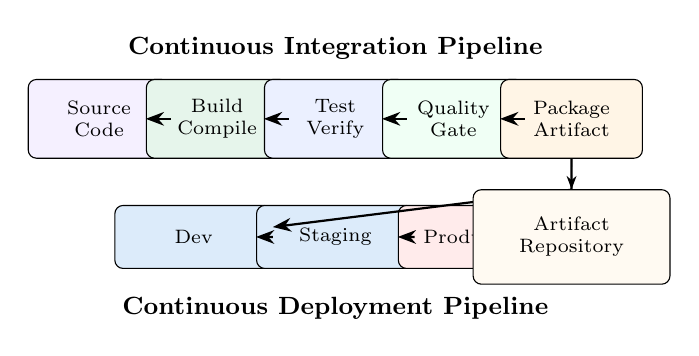
\begin{tikzpicture}[scale=0.6]
        % Pipeline stages
        \node[draw, fill=sourcecolor, rounded corners=3pt, minimum width=1.8cm, minimum height=1cm, font=\scriptsize, align=center] (source) at (-5, 0) {Source\\Code};
        
        \node[draw, fill=pipelinecolor, rounded corners=3pt, minimum width=1.8cm, minimum height=1cm, font=\scriptsize, align=center] (build) at (-2.5, 0) {Build\\Compile};
        
        \node[draw, fill=testcolor, rounded corners=3pt, minimum width=1.8cm, minimum height=1cm, font=\scriptsize, align=center] (test) at (0, 0) {Test\\Verify};
        
        \node[draw, fill=qualitycolor, rounded corners=3pt, minimum width=1.8cm, minimum height=1cm, font=\scriptsize, align=center] (quality) at (2.5, 0) {Quality\\Gate};
        
        \node[draw, fill=artifactcolor, rounded corners=3pt, minimum width=1.8cm, minimum height=1cm, font=\scriptsize, align=center] (artifact) at (5, 0) {Package\\Artifact};
        
        % Arrows
        \draw[-{Stealth}, thick] (source) -- (build);
        \draw[-{Stealth}, thick] (build) -- (test);
        \draw[-{Stealth}, thick] (test) -- (quality);
        \draw[-{Stealth}, thick] (quality) -- (artifact);
        
        % Pipeline label
        \node[font=\small\bfseries] at (0, 1.5) {Continuous Integration Pipeline};
        
        % Deployment stages below
        \node[draw, fill=stagecolor, rounded corners=3pt, minimum width=2cm, minimum height=0.8cm, font=\scriptsize, align=center] (dev) at (-3, -2.5) {Dev};
        
        \node[draw, fill=stagecolor, rounded corners=3pt, minimum width=2cm, minimum height=0.8cm, font=\scriptsize, align=center] (staging) at (0, -2.5) {Staging};
        
        \node[draw, fill=deploycolor, rounded corners=3pt, minimum width=2cm, minimum height=0.8cm, font=\scriptsize, align=center] (prod) at (3, -2.5) {Production};
        
        % Deployment arrows
        \draw[-{Stealth}, thick] (artifact) -- (5, -1.5) -- (dev);
        \draw[-{Stealth}, thick] (dev) -- (staging);
        \draw[-{Stealth}, thick] (staging) -- (prod);
        
        % CD label
        \node[font=\small\bfseries] at (0, -4) {Continuous Deployment Pipeline};
        
        % Artifact repository
        \node[draw, fill=artifactcolor!50, rounded corners=3pt, minimum width=2.5cm, minimum height=1.2cm, font=\scriptsize, align=center] (repo) at (5, -2.5) {Artifact\\Repository};
        \draw[-{Stealth}, dashed] (artifact) -- (repo);
        
    \end{tikzpicture}
    
    \vspace{1.3cm}
    
    \begin{tabular}{ll}
        \textbf{Version:} & 2.0 \\
        \textbf{Status:} & Release \\
        \textbf{Classification:} & ISO/IEC/IEEE 42010 Compliant \\
        \textbf{Last Updated:} & \today \\
    \end{tabular}
    
    \vfill
    
    {\small Based on the Views and Beyond approach to software architecture documentation}
    
\end{titlepage}

\hypersetup{pageanchor=true}
\setcounter{page}{1}

% -----------------------------------------------------------------------------
% TABLE OF CONTENTS
% -----------------------------------------------------------------------------
\tableofcontents
\newpage

% =============================================================================
% SECTION: VIEWPOINT NAME
% =============================================================================
\section{Viewpoint Name}

\begin{definitionbox}[Viewpoint Identification]
\begin{tabular}{@{}L{3.5cm}L{10cm}@{}}
\textbf{Name:} & Builder's View \\[0.5em]
\textbf{Synonyms:} & Build View, CI/CD View, Pipeline View, Integration View, Automation View, DevOps View \\[0.5em]
\textbf{Identifier:} & VP-BLD-001 \\[0.5em]
\textbf{Version:} & 2.0 \\
\end{tabular}
\end{definitionbox}

\subsection{Viewpoint Classification}

The Builder's View addresses the concerns of build engineers, DevOps practitioners, and release managers who need to understand how source code is transformed into deployable artifacts. This viewpoint focuses on automation, continuous integration, continuous delivery, and the quality gates that ensure software readiness.

\begin{table}[H]
\centering
\caption{Viewpoint Classification Taxonomy}
\begin{tabular}{@{}L{4cm}L{10cm}@{}}
\toprule
\textbf{Attribute} & \textbf{Value} \\
\midrule
Style Family & Allocation (Build and CI/CD) \\
Primary Focus & Build Processes, Pipelines, and Automation \\
Abstraction Level & Process / Automation \\
Temporal Perspective & Build-time and Integration-time \\
Related Styles & Development View, Deployment View \\
IEEE 42010 Category & Development Viewpoint (build aspects) \\
DevOps Alignment & Continuous Integration, Continuous Delivery \\
\bottomrule
\end{tabular}
\end{table}

\subsection{Viewpoint Scope}

The Builder's View encompasses the following aspects:

\begin{itemize}
    \item \textbf{Build Systems:} Tools and configurations for compiling and packaging code.
    
    \item \textbf{CI/CD Pipelines:} Automated workflows for integration and delivery.
    
    \item \textbf{Quality Gates:} Automated checks ensuring code quality and standards.
    
    \item \textbf{Artifact Management:} Storage, versioning, and distribution of build outputs.
    
    \item \textbf{Dependency Management:} External library and package handling.
    
    \item \textbf{Environment Configuration:} Build and test environment specifications.
    
    \item \textbf{Release Management:} Versioning, tagging, and release processes.
    
    \item \textbf{Build Performance:} Optimization and efficiency of build processes.
\end{itemize}

% =============================================================================
% SECTION: OVERVIEW
% =============================================================================
\section{Overview}

The Builder's View provides DevOps engineers and developers with comprehensive documentation of how software is built, tested, and prepared for deployment. It ensures consistent, repeatable, and automated software delivery.

\subsection{Purpose and Scope}

The primary purpose of this viewpoint is to document the complete build and integration process, ensuring that anyone can understand, maintain, and improve the CI/CD infrastructure.

\begin{definitionbox}[Viewpoint Definition]
The Builder's View documents the build systems, CI/CD pipelines, quality gates, artifact management, dependency handling, and release processes that transform source code into deployable software. It provides the knowledge needed to maintain reliable, efficient, and automated software delivery infrastructure.
\end{definitionbox}

\subsection{Key Characteristics}

The Builder's View exhibits several distinctive characteristics:

\textbf{Automation-Centric:} Emphasizes automated, repeatable processes over manual steps.

\textbf{Pipeline-Oriented:} Organizes build activities as sequential or parallel pipeline stages.

\textbf{Quality-Focused:} Integrates quality gates and automated verification throughout.

\textbf{Reproducible:} Ensures builds are deterministic and reproducible.

\textbf{Observable:} Provides visibility into build status, metrics, and history.

\subsection{Relationship to Other Viewpoints}

The Builder's View connects to other architectural viewpoints:

\begin{table}[H]
\centering
\caption{Relationships to Other Viewpoints}
\begin{tabular}{@{}L{3.5cm}L{10.5cm}@{}}
\toprule
\textbf{Viewpoint} & \textbf{Relationship} \\
\midrule
Development & Build processes compile module structure. Dependencies defined in development are resolved during build. \\
\addlinespace
Deployment & Build produces deployment artifacts. Pipelines trigger deployment processes. \\
\addlinespace
Operational & Build metrics feed operational dashboards. Build failures trigger alerts. \\
\addlinespace
Designer & Code standards enforced by build quality gates. Patterns verified by static analysis. \\
\addlinespace
Information & Data migrations may be part of release pipeline. Schema changes versioned with artifacts. \\
\addlinespace
Security & Security scanning integrated in pipeline. Secrets management for build processes. \\
\bottomrule
\end{tabular}
\end{table}

\subsection{Build Pipeline Overview}

\begin{figure}[H]
\centering
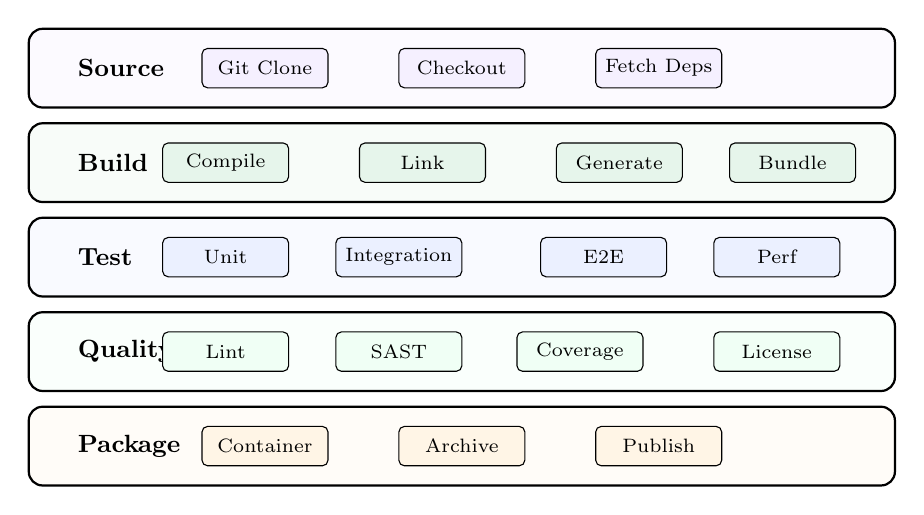
\begin{tikzpicture}[
    node distance=0.8cm and 1.2cm,
    stage/.style={draw, thick, rounded corners=5pt, minimum width=11cm, minimum height=1cm, font=\small},
    element/.style={draw, rounded corners=2pt, minimum width=1.6cm, minimum height=0.5cm, font=\scriptsize},
]
    % Stages
    \node[stage, fill=sourcecolor!30] (source) at (0, 4) {};
    \node[font=\small\bfseries, anchor=west] at (-5, 4) {Source};
    
    \node[stage, fill=pipelinecolor!30] (build) at (0, 2.8) {};
    \node[font=\small\bfseries, anchor=west] at (-5, 2.8) {Build};
    
    \node[stage, fill=testcolor!30] (test) at (0, 1.6) {};
    \node[font=\small\bfseries, anchor=west] at (-5, 1.6) {Test};
    
    \node[stage, fill=qualitycolor!30] (quality) at (0, 0.4) {};
    \node[font=\small\bfseries, anchor=west] at (-5, 0.4) {Quality};
    
    \node[stage, fill=artifactcolor!30] (package) at (0, -0.8) {};
    \node[font=\small\bfseries, anchor=west] at (-5, -0.8) {Package};
    
    % Source elements
    \node[element, fill=sourcecolor] at (-2.5, 4) {Git Clone};
    \node[element, fill=sourcecolor] at (0, 4) {Checkout};
    \node[element, fill=sourcecolor] at (2.5, 4) {Fetch Deps};
    
    % Build elements
    \node[element, fill=pipelinecolor] at (-3, 2.8) {Compile};
    \node[element, fill=pipelinecolor] at (-0.5, 2.8) {Link};
    \node[element, fill=pipelinecolor] at (2, 2.8) {Generate};
    \node[element, fill=pipelinecolor] at (4.2, 2.8) {Bundle};
    
    % Test elements
    \node[element, fill=testcolor] at (-3, 1.6) {Unit};
    \node[element, fill=testcolor] at (-0.8, 1.6) {Integration};
    \node[element, fill=testcolor] at (1.8, 1.6) {E2E};
    \node[element, fill=testcolor] at (4, 1.6) {Perf};
    
    % Quality elements
    \node[element, fill=qualitycolor] at (-3, 0.4) {Lint};
    \node[element, fill=qualitycolor] at (-0.8, 0.4) {SAST};
    \node[element, fill=qualitycolor] at (1.5, 0.4) {Coverage};
    \node[element, fill=qualitycolor] at (4, 0.4) {License};
    
    % Package elements
    \node[element, fill=artifactcolor] at (-2.5, -0.8) {Container};
    \node[element, fill=artifactcolor] at (0, -0.8) {Archive};
    \node[element, fill=artifactcolor] at (2.5, -0.8) {Publish};
    
\end{tikzpicture}
\caption{CI Pipeline Stage Overview}
\end{figure}

% =============================================================================
% SECTION: CONCERNS
% =============================================================================
\section{Concerns}

This section enumerates the build and integration concerns that the Builder's View addresses.

\subsection{Primary Concerns}

\begin{enumerate}[label=\textbf{C\arabic*:}, leftmargin=2.5em]
    \item \textbf{Build System Configuration}
    \begin{itemize}[nosep]
        \item What build tools are used?
        \item How is the build configured?
        \item What are the build targets?
        \item How are build variants managed?
        \item What build optimizations exist?
    \end{itemize}
    
    \item \textbf{CI/CD Pipeline Design}
    \begin{itemize}[nosep]
        \item What pipeline stages exist?
        \item How do stages relate and depend?
        \item What triggers pipeline execution?
        \item What parallel execution exists?
        \item How are failures handled?
    \end{itemize}
    
    \item \textbf{Quality Gate Definition}
    \begin{itemize}[nosep]
        \item What quality checks are automated?
        \item What thresholds must be met?
        \item What happens when gates fail?
        \item How are gate results reported?
        \item How are exceptions handled?
    \end{itemize}
    
    \item \textbf{Artifact Management}
    \begin{itemize}[nosep]
        \item What artifacts are produced?
        \item Where are artifacts stored?
        \item How are artifacts versioned?
        \item What retention policies exist?
        \item How are artifacts promoted?
    \end{itemize}
    
    \item \textbf{Dependency Management}
    \begin{itemize}[nosep]
        \item What dependencies are required?
        \item How are versions specified?
        \item How is dependency resolution handled?
        \item What security scanning exists?
        \item How are updates managed?
    \end{itemize}
    
    \item \textbf{Environment Configuration}
    \begin{itemize}[nosep]
        \item What build environments exist?
        \item How are environments provisioned?
        \item What environment variables are needed?
        \item How is configuration managed?
        \item How is environment parity ensured?
    \end{itemize}
    
    \item \textbf{Release Management}
    \begin{itemize}[nosep]
        \item How are releases versioned?
        \item What is the release branching strategy?
        \item How are release notes generated?
        \item What approval processes exist?
        \item How are hotfixes handled?
    \end{itemize}
    
    \item \textbf{Build Performance}
    \begin{itemize}[nosep]
        \item What is the current build time?
        \item What caching strategies exist?
        \item How is incremental building done?
        \item What parallelization exists?
        \item What are performance targets?
    \end{itemize}
    
    \item \textbf{Security and Secrets}
    \begin{itemize}[nosep]
        \item How are secrets managed?
        \item What security scanning is done?
        \item How is access controlled?
        \item What audit trails exist?
        \item How are vulnerabilities handled?
    \end{itemize}
    
    \item \textbf{Build Observability}
    \begin{itemize}[nosep]
        \item What metrics are collected?
        \item How is build status communicated?
        \item What dashboards exist?
        \item How are trends analyzed?
        \item What alerting exists?
    \end{itemize}
\end{enumerate}

\subsection{Concern-Quality Attribute Mapping}

\begin{table}[H]
\centering
\caption{Concern to Quality Attribute Mapping}
\small
\begin{tabular}{@{}L{2.8cm}C{1cm}C{1cm}C{1cm}C{1cm}C{1cm}C{1cm}C{1cm}C{1cm}@{}}
\toprule
\textbf{Concern} & \rotatebox{60}{\textbf{Reliabil.}} & \rotatebox{60}{\textbf{Effictic.}} & \rotatebox{60}{\textbf{Security}} & \rotatebox{60}{\textbf{Maintain.}} & \rotatebox{60}{\textbf{Traceab.}} & \rotatebox{60}{\textbf{Reproduc.}} & \rotatebox{60}{\textbf{Scalabil.}} & \rotatebox{60}{\textbf{Automat.}} \\
\midrule
Build System & $\bullet$ & $\bullet$ & $\circ$ & $\bullet$ & $\circ$ & $\bullet$ & $\circ$ & $\bullet$ \\
Pipelines & $\bullet$ & $\bullet$ & $\circ$ & $\bullet$ & $\circ$ & $\circ$ & $\bullet$ & $\bullet$ \\
Quality Gates & $\bullet$ & $\circ$ & $\bullet$ & $\bullet$ & $\bullet$ & -- & -- & $\bullet$ \\
Artifacts & $\circ$ & $\circ$ & $\circ$ & $\circ$ & $\bullet$ & $\bullet$ & $\circ$ & $\circ$ \\
Dependencies & $\bullet$ & $\circ$ & $\bullet$ & $\bullet$ & $\bullet$ & $\bullet$ & -- & $\circ$ \\
Environment & $\bullet$ & $\circ$ & $\circ$ & $\circ$ & $\circ$ & $\bullet$ & $\bullet$ & $\circ$ \\
Release Mgmt & $\circ$ & $\circ$ & $\circ$ & $\circ$ & $\bullet$ & $\circ$ & -- & $\circ$ \\
Performance & -- & $\bullet$ & -- & $\circ$ & -- & -- & $\bullet$ & $\circ$ \\
Security & $\circ$ & -- & $\bullet$ & $\circ$ & $\bullet$ & -- & -- & $\bullet$ \\
Observability & $\bullet$ & $\circ$ & $\circ$ & $\bullet$ & $\bullet$ & -- & $\circ$ & $\bullet$ \\
\bottomrule
\multicolumn{9}{l}{\footnotesize $\bullet$ = Primary impact, $\circ$ = Secondary impact, -- = Minimal impact}
\end{tabular}
\end{table}

% =============================================================================
% SECTION: ANTI-CONCERNS
% =============================================================================
\section{Anti-Concerns}

Understanding what the Builder's View is \emph{not} appropriate for helps stakeholders avoid misapplying this viewpoint.

\subsection{Out of Scope Topics}

\begin{enumerate}[label=\textbf{AC\arabic*:}, leftmargin=2.5em]
    \item \textbf{Runtime System Behavior}
    \begin{itemize}[nosep]
        \item Application logic and behavior
        \item Runtime performance characteristics
        \item User interactions
        \item Business process flows
        \item Runtime error handling
    \end{itemize}
    
    \item \textbf{Production Operations}
    \begin{itemize}[nosep]
        \item Production monitoring
        \item Incident management
        \item Capacity planning
        \item Production troubleshooting
        \item SLA management
    \end{itemize}
    
    \item \textbf{Code Design Details}
    \begin{itemize}[nosep]
        \item Design patterns implementation
        \item Algorithm specifics
        \item API design
        \item Data structures
        \item Business logic
    \end{itemize}
    
    \item \textbf{Infrastructure Management}
    \begin{itemize}[nosep]
        \item Production infrastructure
        \item Network configuration
        \item Storage management
        \item Disaster recovery
        \item Infrastructure scaling
    \end{itemize}
    
    \item \textbf{Business Requirements}
    \begin{itemize}[nosep]
        \item Feature specifications
        \item User stories
        \item Business rules
        \item Acceptance criteria
        \item Product roadmap
    \end{itemize}
\end{enumerate}

\begin{warningbox}[Common Misapplications]
Avoid using the Builder's View for:

\begin{itemize}[nosep]
    \item Runtime behavior documentation (use C\&C View)
    \item Production operations (use Operational View)
    \item Code structure (use Development View)
    \item Infrastructure details (use Deployment View)
    \item Design decisions (use Designer's View)
\end{itemize}
\end{warningbox}

% =============================================================================
% SECTION: TYPICAL STAKEHOLDERS
% =============================================================================
\section{Typical Stakeholders}

The Builder's View serves stakeholders involved in software build and delivery automation.

\subsection{Primary Stakeholders}

\begin{table}[H]
\centering
\caption{Primary Stakeholder Analysis}
\small
\begin{tabular}{@{}L{2.6cm}L{3.6cm}L{7cm}@{}}
\toprule
\textbf{Stakeholder} & \textbf{Role Description} & \textbf{Primary Interests} \\
\midrule
DevOps Engineers & Build and maintain CI/CD & Pipeline design, automation, reliability \\
\addlinespace
Build Engineers & Manage build systems & Build optimization, tooling, caching \\
\addlinespace
Release Managers & Coordinate releases & Version control, release process, artifacts \\
\addlinespace
Platform Engineers & Provide build platforms & Environment provisioning, scaling, tools \\
\addlinespace
Security Engineers & Secure the pipeline & Security scanning, secrets, compliance \\
\addlinespace
QA Engineers & Define quality gates & Test automation, coverage, gate criteria \\
\bottomrule
\end{tabular}
\end{table}

\subsection{Secondary Stakeholders}

\begin{table}[H]
\centering
\caption{Secondary Stakeholder Analysis}
\small
\begin{tabular}{@{}L{2.6cm}L{3.6cm}L{7cm}@{}}
\toprule
\textbf{Stakeholder} & \textbf{Role Description} & \textbf{Primary Interests} \\
\midrule
Developers & Write and commit code & Build feedback, local builds, debugging \\
\addlinespace
Tech Leads & Guide technical decisions & Build standards, tooling choices \\
\addlinespace
Architects & Define system structure & Build architecture, dependencies \\
\addlinespace
Product Managers & Plan releases & Release timing, version management \\
\addlinespace
Operations Team & Receive deployments & Artifact quality, deployment readiness \\
\addlinespace
Compliance Officers & Ensure compliance & Audit trails, security compliance \\
\bottomrule
\end{tabular}
\end{table}

\subsection{Stakeholder Concern Matrix}

\begin{table}[H]
\centering
\caption{Stakeholder-Concern Responsibility Matrix}
\footnotesize
\begin{tabular}{@{}L{2cm}C{0.8cm}C{0.8cm}C{0.8cm}C{0.8cm}C{0.8cm}C{0.8cm}C{0.8cm}C{0.8cm}C{0.8cm}C{0.8cm}@{}}
\toprule
& \rotatebox{60}{\textbf{Build Sys}} & \rotatebox{60}{\textbf{Pipelines}} & \rotatebox{60}{\textbf{Quality}} & \rotatebox{60}{\textbf{Artifacts}} & \rotatebox{60}{\textbf{Deps}} & \rotatebox{60}{\textbf{Environ.}} & \rotatebox{60}{\textbf{Release}} & \rotatebox{60}{\textbf{Perform.}} & \rotatebox{60}{\textbf{Security}} & \rotatebox{60}{\textbf{Observ.}} \\
\midrule
DevOps Eng & R & R & C & R & C & R & R & R & C & R \\
Build Eng & R & C & I & C & R & C & I & R & I & C \\
Release Mgr & I & C & C & R & I & I & R & I & C & C \\
Platform Eng & C & C & I & C & C & R & I & C & C & R \\
Security Eng & I & C & R & C & R & C & C & I & R & C \\
QA Engineer & I & C & R & I & I & I & C & I & I & C \\
\bottomrule
\multicolumn{11}{l}{\footnotesize R = Responsible, A = Accountable, C = Consulted, I = Informed}
\end{tabular}
\end{table}

% =============================================================================
% SECTION: MODEL TYPES
% =============================================================================
\section{Model Types}

The Builder's View employs several complementary model types to capture build and integration knowledge.

\subsection{Model Type Catalog}

\begin{enumerate}[label=\textbf{MT\arabic*:}, leftmargin=2.5em]
    \item \textbf{Pipeline Definition}
    \begin{itemize}[nosep]
        \item \textit{Purpose:} Document CI/CD pipeline structure
        \item \textit{Primary Elements:} Stages, jobs, steps, triggers
        \item \textit{Key Relationships:} Depends-on, triggers
        \item \textit{Typical Notation:} YAML, pipeline diagrams
    \end{itemize}
    
    \item \textbf{Build Configuration}
    \begin{itemize}[nosep]
        \item \textit{Purpose:} Specify build system settings
        \item \textit{Primary Elements:} Targets, dependencies, options
        \item \textit{Key Relationships:} Depends-on, produces
        \item \textit{Typical Notation:} Build files (Makefile, Gradle, etc.)
    \end{itemize}
    
    \item \textbf{Artifact Manifest}
    \begin{itemize}[nosep]
        \item \textit{Purpose:} Document build outputs
        \item \textit{Primary Elements:} Artifacts, versions, locations
        \item \textit{Key Relationships:} Produces, stored-in
        \item \textit{Typical Notation:} Manifest files, tables
    \end{itemize}
    
    \item \textbf{Dependency Graph}
    \begin{itemize}[nosep]
        \item \textit{Purpose:} Show dependency relationships
        \item \textit{Primary Elements:} Packages, versions, relationships
        \item \textit{Key Relationships:} Depends-on, conflicts-with
        \item \textit{Typical Notation:} Dependency diagrams, lock files
    \end{itemize}
    
    \item \textbf{Quality Gate Specification}
    \begin{itemize}[nosep]
        \item \textit{Purpose:} Define quality criteria
        \item \textit{Primary Elements:} Checks, thresholds, actions
        \item \textit{Key Relationships:} Requires, blocks
        \item \textit{Typical Notation:} Gate definitions, tables
    \end{itemize}
    
    \item \textbf{Environment Specification}
    \begin{itemize}[nosep]
        \item \textit{Purpose:} Define build environments
        \item \textit{Primary Elements:} Containers, tools, configurations
        \item \textit{Key Relationships:} Runs-on, requires
        \item \textit{Typical Notation:} Dockerfiles, environment configs
    \end{itemize}
    
    \item \textbf{Release Plan}
    \begin{itemize}[nosep]
        \item \textit{Purpose:} Document release process
        \item \textit{Primary Elements:} Versions, branches, approvals
        \item \textit{Key Relationships:} Promotes-to, requires
        \item \textit{Typical Notation:} Release workflows, diagrams
    \end{itemize}
    
    \item \textbf{Build Metrics Dashboard}
    \begin{itemize}[nosep]
        \item \textit{Purpose:} Track build health and performance
        \item \textit{Primary Elements:} Metrics, trends, alerts
        \item \textit{Key Relationships:} Measures, indicates
        \item \textit{Typical Notation:} Dashboards, charts
    \end{itemize}
    
    \item \textbf{Security Scan Report}
    \begin{itemize}[nosep]
        \item \textit{Purpose:} Document security findings
        \item \textit{Primary Elements:} Vulnerabilities, severities, remediation
        \item \textit{Key Relationships:} Affects, remediated-by
        \item \textit{Typical Notation:} Security reports, tables
    \end{itemize}
\end{enumerate}

\subsection{Model Type Relationships}

\begin{figure}[H]
\centering
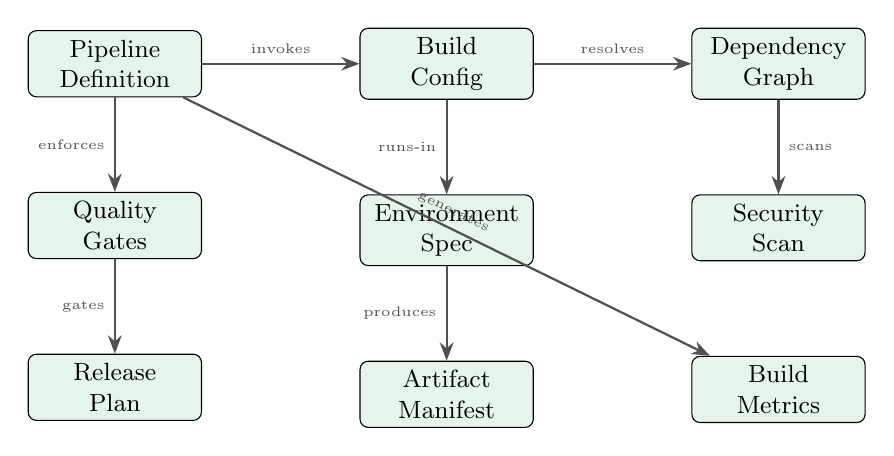
\begin{tikzpicture}[
    node distance=1.2cm and 2cm,
    model/.style={draw, fill=pipelinecolor, rounded corners=3pt, minimum width=2.2cm, minimum height=0.7cm, font=\small, align=center},
    arrow/.style={-{Stealth}, thick, darkgray}
]
    % Nodes - top row
    \node[model] (pipeline) {Pipeline\\Definition};
    \node[model, right=2cm of pipeline] (build) {Build\\Config};
    \node[model, right=2cm of build] (deps) {Dependency\\Graph};
    
    % Nodes - middle row
    \node[model, below=1.2cm of pipeline] (quality) {Quality\\Gates};
    \node[model, below=1.2cm of build] (env) {Environment\\Spec};
    \node[model, below=1.2cm of deps] (security) {Security\\Scan};
    
    % Nodes - bottom row
    \node[model, below=1.2cm of quality] (release) {Release\\Plan};
    \node[model, below=1.2cm of env] (artifact) {Artifact\\Manifest};
    \node[model, below=1.2cm of security] (metrics) {Build\\Metrics};
    
    % Arrows
    \draw[arrow] (pipeline) -- (build) node[midway, above, font=\tiny] {invokes};
    \draw[arrow] (build) -- (deps) node[midway, above, font=\tiny] {resolves};
    \draw[arrow] (pipeline) -- (quality) node[midway, left, font=\tiny] {enforces};
    \draw[arrow] (build) -- (env) node[midway, left, font=\tiny] {runs-in};
    \draw[arrow] (deps) -- (security) node[midway, right, font=\tiny] {scans};
    \draw[arrow] (quality) -- (release) node[midway, left, font=\tiny] {gates};
    \draw[arrow] (env) -- (artifact) node[midway, left, font=\tiny] {produces};
    \draw[arrow] (pipeline) -- (metrics) node[midway, above, sloped, font=\tiny] {generates};
\end{tikzpicture}
\caption{Model Type Dependency Relationships}
\end{figure}

% =============================================================================
% SECTION: MODEL LANGUAGES
% =============================================================================
\section{Model Languages}

For each model type, specific languages, notations, and techniques are prescribed.

\subsection{Pipeline Element Notation}

\begin{figure}[H]
\centering
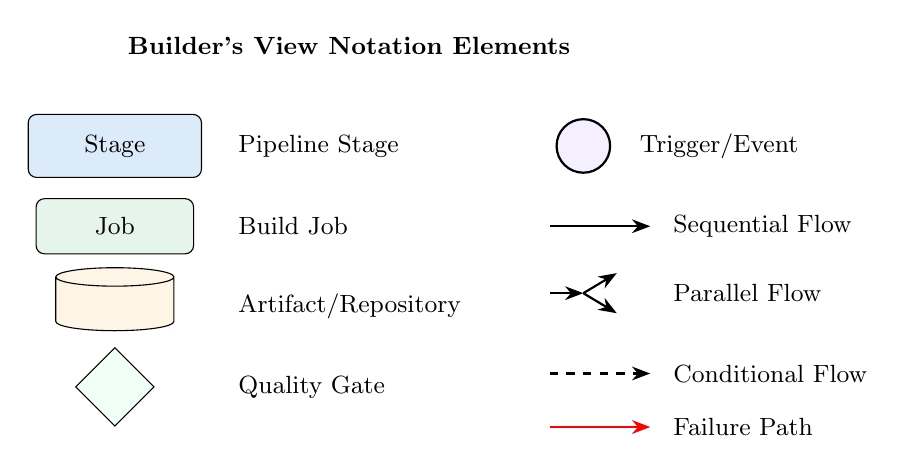
\begin{tikzpicture}[scale=0.85]
    % Legend title
    \node[font=\small\bfseries] at (0, 5) {Builder's View Notation Elements};
    
    % Stage
    \node[draw, fill=stagecolor, rounded corners=3pt, minimum width=2.2cm, minimum height=0.8cm] at (-3.5, 3.5) {};
    \node[font=\small] at (-3.5, 3.5) {Stage};
    \node[right, font=\small] at (-1.8, 3.5) {Pipeline Stage};
    
    % Job
    \node[draw, fill=pipelinecolor, rounded corners=3pt, minimum width=2cm, minimum height=0.7cm] at (-3.5, 2.3) {};
    \node[font=\small] at (-3.5, 2.3) {Job};
    \node[right, font=\small] at (-1.8, 2.3) {Build Job};
    
    % Artifact
    \node[draw, fill=artifactcolor, cylinder, shape border rotate=90, minimum width=1.5cm, minimum height=0.8cm] at (-3.5, 1.1) {};
    \node[right, font=\small] at (-1.8, 1.1) {Artifact/Repository};
    
    % Quality Gate
    \node[draw, fill=qualitycolor, diamond, minimum size=1cm] at (-3.5, -0.1) {};
    \node[right, font=\small] at (-1.8, -0.1) {Quality Gate};
    
    % Trigger
    \draw[thick, fill=sourcecolor] (3.5, 3.5) circle (0.4);
    \node[right, font=\small] at (4.2, 3.5) {Trigger/Event};
    
    % Sequential flow
    \draw[-{Stealth}, thick] (3, 2.3) -- (4.5, 2.3);
    \node[right, font=\small] at (4.7, 2.3) {Sequential Flow};
    
    % Parallel flow
    \draw[-{Stealth}, thick] (3, 1.3) -- (3.5, 1.3);
    \draw[-{Stealth}, thick] (3.5, 1.3) -- (4, 1.6);
    \draw[-{Stealth}, thick] (3.5, 1.3) -- (4, 1);
    \node[right, font=\small] at (4.7, 1.3) {Parallel Flow};
    
    % Conditional
    \draw[-{Stealth}, thick, dashed] (3, 0.1) -- (4.5, 0.1);
    \node[right, font=\small] at (4.7, 0.1) {Conditional Flow};
    
    % Failure
    \draw[-{Stealth}, thick, red] (3, -0.7) -- (4.5, -0.7);
    \node[right, font=\small] at (4.7, -0.7) {Failure Path};
    
\end{tikzpicture}
\caption{Builder's View Notation Legend}
\end{figure}

\subsection{Pipeline Stage Types}

\begin{table}[H]
\centering
\caption{Pipeline Stage Classification}
\small
\begin{tabular}{@{}L{2.5cm}L{4cm}L{6cm}@{}}
\toprule
\textbf{Stage Type} & \textbf{Purpose} & \textbf{Typical Activities} \\
\midrule
Source & Obtain source code & Git clone, checkout, submodules \\
\addlinespace
Build & Compile and link & Compilation, linking, code generation \\
\addlinespace
Test & Verify correctness & Unit tests, integration tests, E2E tests \\
\addlinespace
Quality & Enforce standards & Linting, SAST, coverage, complexity \\
\addlinespace
Security & Scan for vulnerabilities & DAST, dependency scan, secrets scan \\
\addlinespace
Package & Create artifacts & Container build, archive, signing \\
\addlinespace
Publish & Store artifacts & Push to registry, artifact upload \\
\addlinespace
Deploy & Release to environment & Deployment to dev/staging/prod \\
\bottomrule
\end{tabular}
\end{table}

\subsection{Quality Gate Types}

\begin{table}[H]
\centering
\caption{Quality Gate Categories}
\small
\begin{tabular}{@{}L{2.5cm}L{3.5cm}L{3cm}L{3cm}@{}}
\toprule
\textbf{Gate Type} & \textbf{What It Checks} & \textbf{Typical Threshold} & \textbf{Tools} \\
\midrule
Code Coverage & Test coverage percentage & $\geq 80\%$ & JaCoCo, Istanbul \\
\addlinespace
Static Analysis & Code quality issues & 0 critical issues & SonarQube, ESLint \\
\addlinespace
Security Scan & Known vulnerabilities & 0 high/critical CVEs & Snyk, Trivy \\
\addlinespace
License Check & License compliance & Approved licenses only & FOSSA, Black Duck \\
\addlinespace
Performance & Performance regression & $< 10\%$ degradation & JMeter, k6 \\
\addlinespace
Complexity & Code complexity metrics & Cyclomatic $< 10$ & SonarQube \\
\bottomrule
\end{tabular}
\end{table}

\subsection{Artifact Types}

\begin{table}[H]
\centering
\caption{Build Artifact Classification}
\small
\begin{tabular}{@{}L{2.5cm}L{3.5cm}L{3cm}L{3cm}@{}}
\toprule
\textbf{Artifact Type} & \textbf{Description} & \textbf{Storage} & \textbf{Examples} \\
\midrule
Container Image & Docker/OCI images & Container registry & Docker Hub, ECR \\
\addlinespace
Package & Language packages & Package registry & npm, Maven, PyPI \\
\addlinespace
Binary & Compiled executables & Artifact storage & S3, Artifactory \\
\addlinespace
Archive & Compressed bundles & Artifact storage & tar.gz, zip \\
\addlinespace
Documentation & Generated docs & Static hosting & GitHub Pages \\
\addlinespace
Test Results & Test reports & CI storage & JUnit XML, HTML \\
\bottomrule
\end{tabular}
\end{table}

\subsection{Pipeline Configuration Languages}

\begin{table}[H]
\centering
\caption{CI/CD Platform Configuration}
\small
\begin{tabular}{@{}L{2.5cm}L{2.5cm}L{7.5cm}@{}}
\toprule
\textbf{Platform} & \textbf{Config Format} & \textbf{Key Features} \\
\midrule
GitHub Actions & YAML & Workflows, jobs, steps, matrix builds, reusable workflows \\
\addlinespace
GitLab CI & YAML & Stages, jobs, rules, includes, DAG pipelines \\
\addlinespace
Jenkins & Groovy/YAML & Declarative/scripted, shared libraries, plugins \\
\addlinespace
Azure Pipelines & YAML & Stages, jobs, templates, environments, approvals \\
\addlinespace
CircleCI & YAML & Workflows, orbs, executors, caching \\
\addlinespace
Tekton & YAML/K8s & Tasks, pipelines, triggers, Kubernetes-native \\
\bottomrule
\end{tabular}
\end{table}

% =============================================================================
% SECTION: VIEWPOINT METAMODELS
% =============================================================================
\section{Viewpoint Metamodels}

This section defines the conceptual metamodel underlying the Builder's View.

\subsection{Core Metamodel}

\begin{figure}[H]
\centering
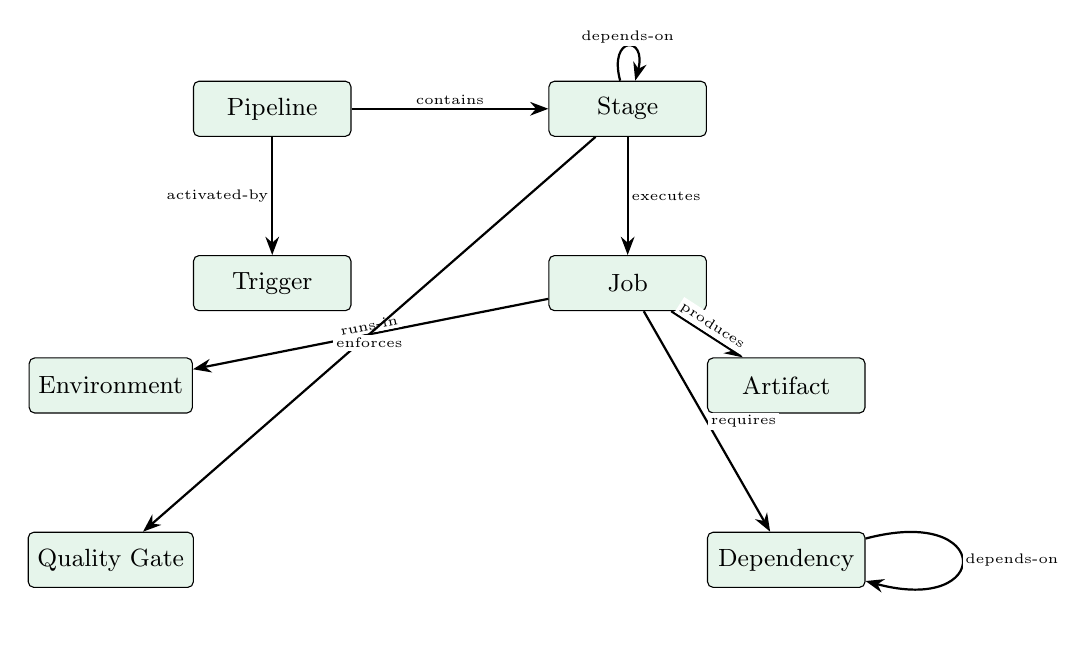
\begin{tikzpicture}[
    node distance=1.3cm and 2cm,
    entity/.style={draw, fill=pipelinecolor, rounded corners=2pt, minimum width=2cm, minimum height=0.7cm, font=\small},
    arrow/.style={-{Stealth}, thick},
    label/.style={font=\tiny, fill=white, inner sep=1pt}
]
    % Main entities
    \node[entity] (pipeline) {Pipeline};
    \node[entity, right=2.5cm of pipeline] (stage) {Stage};
    \node[entity, below=1.5cm of pipeline] (trigger) {Trigger};
    \node[entity, below=1.5cm of stage] (job) {Job};
    \node[entity, below left=2.8cm and 0cm of pipeline] (env) {Environment};
    \node[entity, below right=2.8cm and 0cm of stage] (artifact) {Artifact};
    \node[entity, below=1.5cm of env] (gate) {Quality Gate};
    \node[entity, below=1.5cm of artifact] (dep) {Dependency};
    
    % Relationships
    \draw[arrow] (pipeline) -- (stage) node[label, midway, above] {contains};
    \draw[arrow] (pipeline) -- (trigger) node[label, midway, left] {activated-by};
    \draw[arrow] (stage) -- (job) node[label, midway, right] {executes};
    \draw[arrow] (job) -- (env) node[label, midway, above, sloped] {runs-in};
    \draw[arrow] (job) -- (artifact) node[label, midway, above, sloped] {produces};
    \draw[arrow] (stage) -- (gate) node[label, midway, below] {enforces};
    \draw[arrow] (job) -- (dep) node[label, midway, right] {requires};
    
    % Self-reference
    \draw[arrow] (stage) to[loop above] node[label, above] {depends-on} (stage);
    \draw[arrow] (dep) to[loop right] node[label, right] {depends-on} (dep);
\end{tikzpicture}
\caption{Builder's View Core Metamodel}
\end{figure}

\subsection{Entity Definitions}

\begin{definitionbox}[Entity: Pipeline]
\textbf{Definition:} An automated workflow that orchestrates the build, test, and delivery process.

\textbf{Attributes:}
\begin{itemize}[nosep]
    \item \texttt{pipelineId}: Unique identifier
    \item \texttt{name}: Pipeline name
    \item \texttt{description}: Pipeline purpose
    \item \texttt{triggers}: Events that start the pipeline
    \item \texttt{stages}: Ordered list of stages
    \item \texttt{timeout}: Maximum execution time
    \item \texttt{concurrency}: Parallel execution settings
    \item \texttt{variables}: Pipeline-level variables
    \item \texttt{caching}: Cache configuration
    \item \texttt{notifications}: Alert settings
\end{itemize}

\textbf{Constraints:}
\begin{itemize}[nosep]
    \item Pipeline should have at least one trigger
    \item Pipeline should have at least one stage
    \item Timeout should be reasonable
\end{itemize}
\end{definitionbox}

\begin{definitionbox}[Entity: Stage]
\textbf{Definition:} A logical grouping of jobs that execute together in the pipeline.

\textbf{Attributes:}
\begin{itemize}[nosep]
    \item \texttt{stageId}: Unique identifier
    \item \texttt{name}: Stage name
    \item \texttt{type}: Stage type (build, test, deploy, etc.)
    \item \texttt{jobs}: Jobs in this stage
    \item \texttt{dependencies}: Required previous stages
    \item \texttt{condition}: Execution condition
    \item \texttt{environment}: Target environment
    \item \texttt{approvals}: Required approvals
    \item \texttt{timeout}: Stage timeout
    \item \texttt{retryPolicy}: Retry configuration
\end{itemize}

\textbf{Constraints:}
\begin{itemize}[nosep]
    \item Dependencies must not create cycles
    \item Stages should have clear purposes
    \item Conditions should be deterministic
\end{itemize}
\end{definitionbox}

\begin{definitionbox}[Entity: Job]
\textbf{Definition:} A unit of work executed on a build agent, consisting of steps.

\textbf{Attributes:}
\begin{itemize}[nosep]
    \item \texttt{jobId}: Unique identifier
    \item \texttt{name}: Job name
    \item \texttt{steps}: Ordered list of steps
    \item \texttt{environment}: Execution environment
    \item \texttt{agent}: Build agent requirements
    \item \texttt{matrix}: Matrix build parameters
    \item \texttt{services}: Required services (databases, etc.)
    \item \texttt{artifacts}: Artifacts produced/consumed
    \item \texttt{cache}: Cache configuration
    \item \texttt{timeout}: Job timeout
\end{itemize}

\textbf{Constraints:}
\begin{itemize}[nosep]
    \item Jobs should be atomic and independent where possible
    \item Environment requirements should be explicit
    \item Timeouts should prevent hung jobs
\end{itemize}
\end{definitionbox}

\begin{definitionbox}[Entity: Trigger]
\textbf{Definition:} An event or condition that initiates pipeline execution.

\textbf{Attributes:}
\begin{itemize}[nosep]
    \item \texttt{triggerId}: Unique identifier
    \item \texttt{type}: Trigger type (push, PR, schedule, manual, API)
    \item \texttt{source}: Event source (branch, tag, webhook)
    \item \texttt{filters}: Inclusion/exclusion patterns
    \item \texttt{schedule}: Cron expression for scheduled triggers
    \item \texttt{conditions}: Additional conditions
    \item \texttt{parameters}: Input parameters
    \item \texttt{enabled}: Whether trigger is active
\end{itemize}

\textbf{Constraints:}
\begin{itemize}[nosep]
    \item Triggers should be specific enough to avoid unnecessary builds
    \item Schedule expressions should be valid cron syntax
    \item Filters should cover intended scope
\end{itemize}
\end{definitionbox}

\begin{definitionbox}[Entity: Artifact]
\textbf{Definition:} A build output that is stored, versioned, and potentially deployed.

\textbf{Attributes:}
\begin{itemize}[nosep]
    \item \texttt{artifactId}: Unique identifier
    \item \texttt{name}: Artifact name
    \item \texttt{type}: Artifact type (container, package, binary, etc.)
    \item \texttt{version}: Version identifier
    \item \texttt{checksum}: Integrity hash
    \item \texttt{location}: Storage location
    \item \texttt{metadata}: Additional metadata
    \item \texttt{signature}: Digital signature
    \item \texttt{retention}: Retention policy
    \item \texttt{scanResults}: Security scan results
\end{itemize}

\textbf{Constraints:}
\begin{itemize}[nosep]
    \item Artifacts should be immutable once published
    \item Versions should follow semantic versioning
    \item Checksums should be verified on retrieval
\end{itemize}
\end{definitionbox}

\begin{definitionbox}[Entity: Environment]
\textbf{Definition:} The execution context where build jobs run, including tools and configuration.

\textbf{Attributes:}
\begin{itemize}[nosep]
    \item \texttt{environmentId}: Unique identifier
    \item \texttt{name}: Environment name
    \item \texttt{type}: Environment type (container, VM, bare metal)
    \item \texttt{image}: Container/VM image reference
    \item \texttt{tools}: Installed tools and versions
    \item \texttt{variables}: Environment variables
    \item \texttt{secrets}: Secret references
    \item \texttt{resources}: CPU, memory, storage
    \item \texttt{network}: Network configuration
    \item \texttt{caching}: Cache mounts
\end{itemize}

\textbf{Constraints:}
\begin{itemize}[nosep]
    \item Environments should be reproducible
    \item Secrets should never be logged
    \item Resources should be appropriate for workload
\end{itemize}
\end{definitionbox}

\begin{definitionbox}[Entity: Quality Gate]
\textbf{Definition:} An automated check that must pass before proceeding in the pipeline.

\textbf{Attributes:}
\begin{itemize}[nosep]
    \item \texttt{gateId}: Unique identifier
    \item \texttt{name}: Gate name
    \item \texttt{type}: Gate type (coverage, security, etc.)
    \item \texttt{metric}: What is measured
    \item \texttt{threshold}: Required value
    \item \texttt{operator}: Comparison operator
    \item \texttt{action}: What happens on failure
    \item \texttt{exceptions}: Allowed exceptions
    \item \texttt{evidence}: Documentation of results
    \item \texttt{trend}: Historical trend tracking
\end{itemize}

\textbf{Constraints:}
\begin{itemize}[nosep]
    \item Gates should be objective and measurable
    \item Thresholds should be achievable
    \item Exceptions should be documented and temporary
\end{itemize}
\end{definitionbox}

\begin{definitionbox}[Entity: Dependency]
\textbf{Definition:} An external package or library required by the build.

\textbf{Attributes:}
\begin{itemize}[nosep]
    \item \texttt{dependencyId}: Unique identifier
    \item \texttt{name}: Package name
    \item \texttt{version}: Version constraint
    \item \texttt{resolvedVersion}: Actual resolved version
    \item \texttt{source}: Package registry
    \item \texttt{scope}: Dependency scope (compile, test, runtime)
    \item \texttt{transitive}: Whether transitive or direct
    \item \texttt{license}: License information
    \item \texttt{vulnerabilities}: Known vulnerabilities
    \item \texttt{checksum}: Integrity verification
\end{itemize}

\textbf{Constraints:}
\begin{itemize}[nosep]
    \item Versions should be pinned or use lock files
    \item Licenses should be reviewed
    \item Vulnerabilities should be assessed
\end{itemize}
\end{definitionbox}

\subsection{Relationship Definitions}

\begin{table}[H]
\centering
\caption{Metamodel Relationship Definitions}
\small
\begin{tabular}{@{}L{2.3cm}L{1.8cm}L{1.8cm}L{7.5cm}@{}}
\toprule
\textbf{Relationship} & \textbf{Source} & \textbf{Target} & \textbf{Description} \\
\midrule
contains & Pipeline & Stage & Pipeline includes stages \\
\addlinespace
activated-by & Pipeline & Trigger & Trigger starts pipeline \\
\addlinespace
executes & Stage & Job & Stage runs jobs \\
\addlinespace
runs-in & Job & Environment & Job uses environment \\
\addlinespace
produces & Job & Artifact & Job creates artifact \\
\addlinespace
enforces & Stage & Gate & Stage checks gate \\
\addlinespace
requires & Job & Dependency & Job needs dependency \\
\addlinespace
depends-on & Stage & Stage & Stage ordering \\
\addlinespace
depends-on & Dependency & Dependency & Transitive dependencies \\
\bottomrule
\end{tabular}
\end{table}

% =============================================================================
% SECTION: MODEL CORRESPONDENCE RULES
% =============================================================================
\section{Model Correspondence Rules}

Model correspondence rules define how build elements relate to elements in other views.

\subsection{Development View Correspondence}

\begin{definitionbox}[Correspondence Rule CR-01: Module to Build Target Mapping]
\textbf{Rule:} Each deployable module should have a corresponding build target.

\textbf{Formal Expression:}
\begin{center}
$\forall m \in DeployableModules : \exists t \in BuildTargets : builds(t, m)$
\end{center}

\textbf{Rationale:} Ensures all modules can be built.

\textbf{Verification:} Build target coverage analysis.
\end{definitionbox}

\subsection{Deployment View Correspondence}

\begin{definitionbox}[Correspondence Rule CR-02: Artifact to Deployment Mapping]
\textbf{Rule:} Each deployment target should receive a build artifact.

\textbf{Formal Expression:}
\begin{center}
$\forall d \in DeploymentTargets : \exists a \in Artifacts : deploys(a, d)$
\end{center}

\textbf{Rationale:} Ensures deployment receives build outputs.

\textbf{Verification:} Deployment artifact traceability.
\end{definitionbox}

\subsection{Designer's View Correspondence}

\begin{definitionbox}[Correspondence Rule CR-03: Quality Gate to Standard Mapping]
\textbf{Rule:} Design standards should be enforced by quality gates.

\textbf{Formal Expression:}
\begin{center}
$\forall s \in AutomatableStandards : \exists g \in QualityGates : enforces(g, s)$
\end{center}

\textbf{Rationale:} Automates standards compliance.

\textbf{Verification:} Standards automation coverage.
\end{definitionbox}

% =============================================================================
% SECTION: OPERATIONS ON VIEWS
% =============================================================================
\section{Operations on Views}

This section defines methods for creating, analyzing, and maintaining build views.

\subsection{Creation Methods}

\subsubsection{View Development Process}

\begin{guidancebox}[Step 1: Define Build Targets]
\begin{enumerate}[nosep]
    \item Identify all deployable components
    \item Define build outputs for each
    \item Specify target platforms
    \item Document build variants
    \item Configure build tools
\end{enumerate}
\end{guidancebox}

\begin{guidancebox}[Step 2: Design Pipeline Structure]
\begin{enumerate}[nosep]
    \item Identify pipeline stages
    \item Define stage dependencies
    \item Specify parallel execution opportunities
    \item Configure triggers
    \item Set up notifications
\end{enumerate}
\end{guidancebox}

\begin{guidancebox}[Step 3: Configure Quality Gates]
\begin{enumerate}[nosep]
    \item Identify quality metrics
    \item Set threshold values
    \item Configure gate actions
    \item Document exception process
    \item Set up trend tracking
\end{enumerate}
\end{guidancebox}

\begin{guidancebox}[Step 4: Set Up Artifact Management]
\begin{enumerate}[nosep]
    \item Define artifact types
    \item Configure storage locations
    \item Set versioning scheme
    \item Define retention policies
    \item Configure signing/verification
\end{enumerate}
\end{guidancebox}

\begin{guidancebox}[Step 5: Configure Environments]
\begin{enumerate}[nosep]
    \item Define build environments
    \item Specify required tools
    \item Configure secrets management
    \item Set up caching
    \item Document environment requirements
\end{enumerate}
\end{guidancebox}

\begin{guidancebox}[Step 6: Implement Security]
\begin{enumerate}[nosep]
    \item Configure dependency scanning
    \item Set up SAST/DAST
    \item Implement secrets management
    \item Configure access controls
    \item Set up audit logging
\end{enumerate}
\end{guidancebox}

\begin{guidancebox}[Step 7: Establish Monitoring]
\begin{enumerate}[nosep]
    \item Define key metrics
    \item Set up dashboards
    \item Configure alerts
    \item Plan trend analysis
    \item Document SLOs
\end{enumerate}
\end{guidancebox}

\subsubsection{Pipeline Design Patterns}

\begin{patternbox}[Pattern: Trunk-Based Pipeline]
\textbf{Context:} Continuous integration with short-lived branches.

\textbf{Structure:}
\begin{itemize}[nosep]
    \item Single main branch (trunk)
    \item Feature flags for incomplete features
    \item Automated deployment on merge
    \item Fast feedback loops
\end{itemize}

\textbf{Benefits:} Reduced merge conflicts, faster integration, simpler branching.
\end{patternbox}

\begin{patternbox}[Pattern: Environment Promotion]
\textbf{Context:} Progressive deployment through environments.

\textbf{Structure:}
\begin{itemize}[nosep]
    \item Dev $\rightarrow$ Staging $\rightarrow$ Production
    \item Same artifact promoted through stages
    \item Automated gates between environments
    \item Manual approval for production
\end{itemize}

\textbf{Benefits:} Confidence building, risk reduction, audit trail.
\end{patternbox}

\begin{patternbox}[Pattern: Matrix Build]
\textbf{Context:} Testing across multiple configurations.

\textbf{Structure:}
\begin{itemize}[nosep]
    \item Define configuration matrix (OS, version, etc.)
    \item Parallel execution of combinations
    \item Aggregate results
    \item Fail fast on critical failures
\end{itemize}

\textbf{Benefits:} Comprehensive testing, efficient execution, early detection.
\end{patternbox}

\subsection{Analysis Methods}

\subsubsection{Build Performance Analysis}

\begin{definitionbox}[Build Time Optimization]
\textbf{Purpose:} Identify and eliminate build time bottlenecks.

\textbf{Metrics:}
\begin{itemize}[nosep]
    \item Total pipeline duration
    \item Individual stage/job times
    \item Queue wait time
    \item Cache hit rates
    \item Parallelization efficiency
\end{itemize}

\textbf{Techniques:}
\begin{itemize}[nosep]
    \item Identify critical path
    \item Measure cache effectiveness
    \item Analyze parallelization opportunities
    \item Profile slow steps
    \item Optimize dependency resolution
\end{itemize}
\end{definitionbox}

% =============================================================================
% SECTION: EXAMPLES
% =============================================================================
\section{Examples}

\subsection{Example 1: CI/CD Pipeline Diagram}

\begin{figure}[H]
\centering
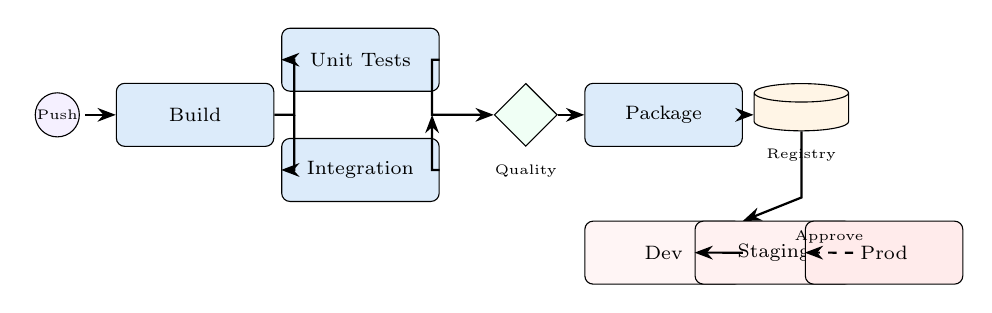
\begin{tikzpicture}[
    stage/.style={draw, fill=stagecolor, rounded corners=3pt, minimum width=2cm, minimum height=0.8cm, font=\scriptsize, align=center},
    gate/.style={draw, fill=qualitycolor, diamond, minimum size=0.8cm, font=\tiny},
    artifact/.style={draw, fill=artifactcolor, cylinder, shape border rotate=90, minimum width=1.2cm, minimum height=0.6cm, font=\tiny},
    scale=0.7
]
    % Trigger
    \draw[fill=sourcecolor] (-5, 0) circle (0.4);
    \node[font=\tiny] at (-5, 0) {Push};
    
    % Build stage
    \node[stage] (build) at (-2.5, 0) {Build};
    
    % Test stages (parallel)
    \node[stage] (unit) at (0.5, 1) {Unit Tests};
    \node[stage] (int) at (0.5, -1) {Integration};
    
    % Quality gate
    \node[gate] (gate) at (3.5, 0) {};
    \node[font=\tiny, below=0.1cm of gate] {Quality};
    
    % Package
    \node[stage] (package) at (6, 0) {Package};
    
    % Artifact
    \node[artifact] (artifact) at (8.5, 0) {};
    \node[font=\tiny, below=0.1cm of artifact] {Registry};
    
    % Deploy stages
    \node[stage, fill=deploycolor!50] (dev) at (6, -2.5) {Dev};
    \node[stage, fill=deploycolor!70] (staging) at (8, -2.5) {Staging};
    \node[stage, fill=deploycolor] (prod) at (10, -2.5) {Prod};
    
    % Arrows
    \draw[-{Stealth}, thick] (-4.5, 0) -- (build);
    \draw[-{Stealth}, thick] (build) -- (-0.7, 0) -- (-0.7, 1) -- (unit);
    \draw[-{Stealth}, thick] (-0.7, 0) -- (-0.7, -1) -- (int);
    \draw[-{Stealth}, thick] (unit) -- (1.8, 1) -- (1.8, 0) -- (gate);
    \draw[-{Stealth}, thick] (int) -- (1.8, -1) -- (1.8, 0);
    \draw[-{Stealth}, thick] (gate) -- (package);
    \draw[-{Stealth}, thick] (package) -- (artifact);
    
    % Deploy arrows
    \draw[-{Stealth}, thick] (artifact) -- (8.5, -1.5) -- (dev);
    \draw[-{Stealth}, thick] (dev) -- (staging);
    \draw[-{Stealth}, dashed, thick] (staging) -- (prod);
    
    % Manual approval
    \node[font=\tiny, above] at (9, -2.5) {Approve};
    
\end{tikzpicture}
\caption{Complete CI/CD Pipeline}
\end{figure}

\textbf{Description:} This diagram shows a complete CI/CD pipeline. A push event triggers the build stage. Unit and integration tests run in parallel. A quality gate checks coverage and security. On success, artifacts are packaged and published to the registry. Deployment proceeds through Dev and Staging automatically, with manual approval required for Production.

\subsection{Example 2: GitHub Actions Workflow}

\begin{lstlisting}[language=yaml, caption=Example GitHub Actions Workflow]
name: CI/CD Pipeline

on:
  push:
    branches: [main, develop]
  pull_request:
    branches: [main]

jobs:
  build:
    runs-on: ubuntu-latest
    steps:
      - uses: actions/checkout@v4
      - uses: actions/setup-node@v4
        with:
          node-version: '20'
          cache: 'npm'
      - run: npm ci
      - run: npm run build
      - uses: actions/upload-artifact@v4
        with:
          name: build-output
          path: dist/

  test:
    needs: build
    runs-on: ubuntu-latest
    strategy:
      matrix:
        test-type: [unit, integration]
    steps:
      - uses: actions/checkout@v4
      - run: npm ci
      - run: npm run test:${{ matrix.test-type }}

  quality:
    needs: test
    runs-on: ubuntu-latest
    steps:
      - uses: actions/checkout@v4
      - run: npm ci
      - run: npm run lint
      - run: npm run test:coverage
      - uses: SonarSource/sonarcloud-github-action@master
\end{lstlisting}

\subsection{Example 3: Quality Gate Configuration}

\begin{table}[H]
\centering
\caption{Quality Gate Definition}
\small
\begin{tabular}{@{}L{2.5cm}L{2.5cm}C{2cm}C{2cm}L{2.5cm}@{}}
\toprule
\textbf{Gate} & \textbf{Metric} & \textbf{Threshold} & \textbf{Current} & \textbf{Action} \\
\midrule
Coverage & Line coverage & $\geq 80\%$ & \cellcolor{green!30}85\% & Block merge \\
\addlinespace
Security & Critical CVEs & 0 & \cellcolor{green!30}0 & Block deploy \\
\addlinespace
Complexity & Cyclomatic & $< 15$ & \cellcolor{green!30}12 & Warning \\
\addlinespace
Duplication & Duplicate code & $< 5\%$ & \cellcolor{yellow!30}4.2\% & Warning \\
\addlinespace
Debt & Tech debt ratio & $< 5\%$ & \cellcolor{green!30}3.1\% & Informational \\
\bottomrule
\end{tabular}
\end{table}

% =============================================================================
% SECTION: NOTES
% =============================================================================
\section{Notes}

\subsection{Pipeline Best Practices}

\begin{pipelinebox}[CI/CD Best Practices]
\begin{itemize}[nosep]
    \item \textbf{Fast Feedback:} Optimize for quick build times; developers need rapid feedback
    \item \textbf{Fail Fast:} Run quick checks first; don't waste time on obvious failures
    \item \textbf{Reproducibility:} Builds should be deterministic and reproducible
    \item \textbf{Immutable Artifacts:} Never modify artifacts after publishing
    \item \textbf{Version Everything:} Code, config, and infrastructure as code
    \item \textbf{Automate Everything:} Manual steps are error-prone and slow
    \item \textbf{Monitor and Alert:} Track build health and alert on degradation
\end{itemize}
\end{pipelinebox}

\subsection{Artifact Management Guidelines}

\begin{artifactbox}[Artifact Best Practices]
\begin{itemize}[nosep]
    \item \textbf{Semantic Versioning:} Use SemVer for meaningful version numbers
    \item \textbf{Integrity Verification:} Sign and verify artifact checksums
    \item \textbf{Retention Policies:} Define how long artifacts are kept
    \item \textbf{Promotion Model:} Same artifact moves through environments
    \item \textbf{Metadata:} Include build info, commit hash, timestamp
    \item \textbf{Cleanup:} Automatically clean old/unused artifacts
\end{itemize}
\end{artifactbox}

\subsection{Common Pitfalls}

\begin{warningbox}[Build Anti-Patterns to Avoid]
\begin{enumerate}[nosep]
    \item \textbf{Snowflake Builds:} Unreproducible builds that work only sometimes
    \item \textbf{Slow Pipelines:} Long build times that discourage frequent commits
    \item \textbf{Flaky Tests:} Tests that fail intermittently, eroding trust
    \item \textbf{Secret Leakage:} Secrets appearing in logs or artifacts
    \item \textbf{Missing Gates:} Skipping quality checks to meet deadlines
    \item \textbf{Manual Steps:} Human intervention required in pipeline
    \item \textbf{Environment Drift:} Build environments differing from production
    \item \textbf{Unversioned Configs:} Pipeline configs not in version control
\end{enumerate}
\end{warningbox}

% =============================================================================
% SECTION: SOURCES
% =============================================================================
\section{Sources}

\subsection{Primary References}

\begin{enumerate}
    \item Humble, J., \& Farley, D. (2010). \textit{Continuous Delivery: Reliable Software Releases through Build, Test, and Deployment Automation}. Addison-Wesley.
    
    \item Kim, G., et al. (2016). \textit{The DevOps Handbook}. IT Revolution Press.
    
    \item Forsgren, N., Humble, J., \& Kim, G. (2018). \textit{Accelerate: The Science of Lean Software and DevOps}. IT Revolution Press.
    
    \item Richardson, C. (2018). \textit{Microservices Patterns}. Manning Publications.
    
    \item Bass, L., Weber, I., \& Zhu, L. (2015). \textit{DevOps: A Software Architect's Perspective}. Addison-Wesley.
\end{enumerate}

\subsection{Supplementary References}

\begin{enumerate}[resume]
    \item Morris, K. (2016). \textit{Infrastructure as Code}. O'Reilly Media.
    
    \item Davis, J., \& Daniels, R. (2016). \textit{Effective DevOps}. O'Reilly Media.
    
    \item Nygard, M. (2018). \textit{Release It!} (2nd ed.). Pragmatic Bookshelf.
    
    \item Beyer, B., et al. (2016). \textit{Site Reliability Engineering}. O'Reilly Media.
    
    \item Martin, R. C. (2008). \textit{Clean Code}. Prentice Hall.
\end{enumerate}

\subsection{Online Resources}

\begin{itemize}
    \item GitHub Actions Documentation: \url{https://docs.github.com/actions}
    \item GitLab CI/CD Documentation: \url{https://docs.gitlab.com/ee/ci/}
    \item Jenkins Documentation: \url{https://www.jenkins.io/doc/}
    \item DORA Metrics: \url{https://dora.dev/}
\end{itemize}

% =============================================================================
% APPENDIX
% =============================================================================
\appendix

\section{Builder's View Checklist}

\begin{table}[H]
\centering
\small
\begin{tabular}{@{}L{10cm}C{2cm}@{}}
\toprule
\textbf{Item} & \textbf{Complete?} \\
\midrule
\multicolumn{2}{l}{\textbf{Build System}} \\
\quad Build targets defined for all components & $\square$ \\
\quad Build configuration in version control & $\square$ \\
\quad Local build possible & $\square$ \\
\quad Build variants documented & $\square$ \\
\midrule
\multicolumn{2}{l}{\textbf{Pipeline}} \\
\quad Pipeline stages defined & $\square$ \\
\quad Triggers configured & $\square$ \\
\quad Parallel execution optimized & $\square$ \\
\quad Failure handling defined & $\square$ \\
\quad Notifications configured & $\square$ \\
\midrule
\multicolumn{2}{l}{\textbf{Quality}} \\
\quad Quality gates defined & $\square$ \\
\quad Thresholds set appropriately & $\square$ \\
\quad Security scanning enabled & $\square$ \\
\quad License compliance checked & $\square$ \\
\midrule
\multicolumn{2}{l}{\textbf{Artifacts}} \\
\quad Artifact types documented & $\square$ \\
\quad Versioning scheme defined & $\square$ \\
\quad Storage configured & $\square$ \\
\quad Retention policies set & $\square$ \\
\midrule
\multicolumn{2}{l}{\textbf{Operations}} \\
\quad Build metrics collected & $\square$ \\
\quad Dashboards created & $\square$ \\
\quad Alerts configured & $\square$ \\
\quad Documentation complete & $\square$ \\
\bottomrule
\end{tabular}
\end{table}

\section{Glossary}

\begin{description}[style=nextline, leftmargin=3cm, labelwidth=2.8cm]
    \item[Artifact] A build output such as a binary, container image, or package.
    
    \item[CI] Continuous Integration; automatically building and testing code changes.
    
    \item[CD] Continuous Delivery/Deployment; automatically releasing software.
    
    \item[DAST] Dynamic Application Security Testing; testing running applications.
    
    \item[Job] A unit of work in a pipeline, executed on a build agent.
    
    \item[Pipeline] An automated workflow for build, test, and deployment.
    
    \item[Quality Gate] An automated check that must pass to proceed.
    
    \item[SAST] Static Application Security Testing; analyzing source code.
    
    \item[SemVer] Semantic Versioning; a versioning scheme (MAJOR.MINOR.PATCH).
    
    \item[Stage] A logical grouping of jobs in a pipeline.
    
    \item[Trigger] An event that initiates pipeline execution.
\end{description}

% =============================================================================
% END DOCUMENT
% =============================================================================

\end{document}
